\chapter{Background}
In this section, we give background on the different concepts and technologies used in this thesis, which include logic-based reasoning Simulink, stochastic timed automata,  statistical model checking, integer-linear programming and population-based metaheuristics.
\section{Logic-based Reasoning}
In this thesis, we express requirements specifications in  Boolean logic and apply \textit{Boolean satisfiability} (SAT) to detect inconsistencies within the specifications. Furthermore, we use \textit{ontology} to represent the specifications, and conduct rigorous analysis via a linguistic approach.
\subsection*{Boolean Satisfiability}
The study of a Boolean formula is generally concerned with the set of truth assignments (assignments of 0 or 1 to each of the variables) that make the formula true. Finding such assignments by answering the simpler question: ``does there exist a truth assignment that satisfies the Boolean formula?'' is called the Boolean satisfiability problem (SAT), which is proven to be NP complete~\cite{devlin2008satisfiability}\cite{Biere2009HandbookSatisfiability}. However, efficient heuristics and approximation algorithms do exist to solve such problems.

SAT problems are usually checked using decision procedures known as SAT solvers. Z3 integrates several background theories (or Satisfiability Module Theories, SMT) and decision procedures based on SAT solvers~\cite{DeMoura2008Z3:Solver}. It is a well known SMT solver and a theorem prover developed by Microsoft Research which has been used in the formal verification and reasoning of software and hardware systems, mainly due to its strong support for integration to verification tools via its well known APIs written in Java, Phyton, C++, C and .Net. 

Z3's input language is an extension of the SMT-LIB2 standard, which are commands used to assert logical statements and instruct the solver to do some action, e.g., to check for satisfiability, the command \textit{(check-sat) }is envoked. Z3 returns \textit{sat} if the formulas are satisfiable. If the formulas are not satisfiable, Z3 returns \textit{unsat}, or if it cannot decide the result, it returns \textit{unknown}. In case of unsat, if the unsat-core option is enabled, Z3 can return the subset of unsatisfiable assertions by envoking the \textit{(get-unsat-core)} command.

\subsection*{Ontology and Description Logic}
Ontology is a knowledge representation technique frequently used in the artificial intelligence and other domains to facilitate automated decision making. It is defined as ``a formal specification of a shared conceptualization'' according to Borst \cite{Borst1997ConstructionOntologies}. It employs different modeling entities, e.g., concepts, instances, axioms, which are compared to classes, objects, inheritance in Object-Oriented Progreamming. The ontology is consistent if every axioms and relations (or assertions) hold~\cite{Mankovskii2009OWL:Language}.

Description logic (DL)~\cite{Baader2010TheApplications} is a knowledge presentation language, and is the most widely language used to construct ontologies. It is a fragment of first-order logic with many of the core reasoning problems decidable. For this reason, it has several application, e.g., in web semantics (e.g., OWL)~\cite{conf/owled/ShearerMH08}, artificial intelligence~\cite{10.1007/978-94-017-9297-4_7}, bioinformatics~\cite{Rector2006}, software engineering, natural language processing. Thus, it is usually backed by solid reasoning services that terminate and deliver results in reasonable time. 

\section{Simulink}
Simulink~\cite{JamesB.Dabney2003MasteringSimulink} is a graphical development environment for the modeling, simulation and analysis of embedded systems which is widely used in industry to model and inspect the dynamics of systems before implementation. It is robust as it supports multi-domain, continuous, discrete, hybrid systems, also discrete systems that execute with different sampling times (or multi-rate). Figure~\ref{fig_sm_multi-rate} shows a multi-rate subsystem of the brake-by-wire Simulink model that models the brake pedal (i.e., continuous behavior) and global brake functionality (i.e., discrete behavior), which executes every 10ms and 20ms.  
\begin{figure}[h]
	\centering
	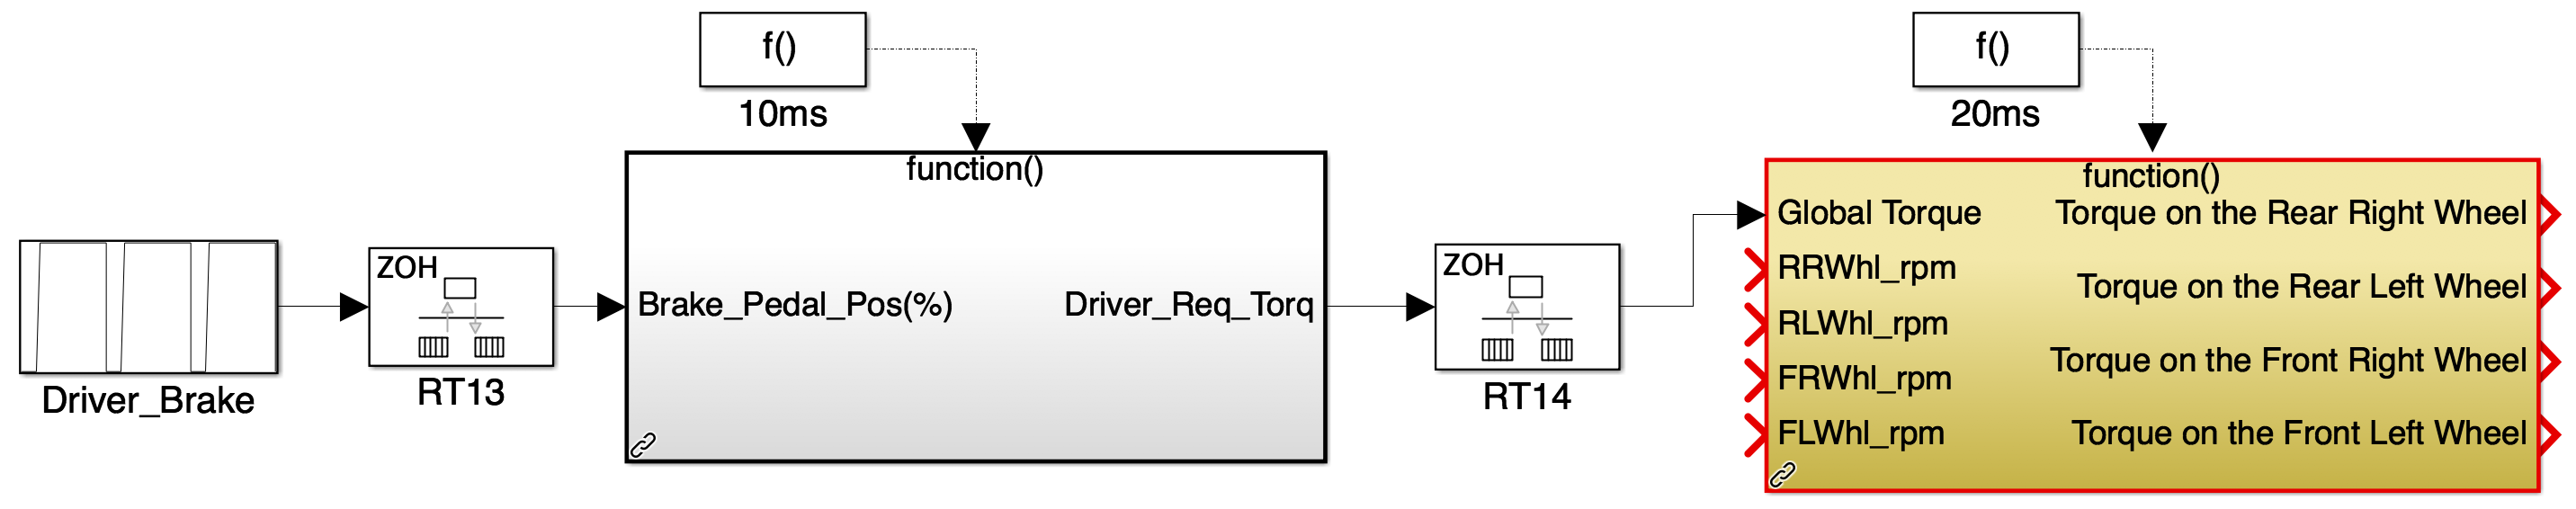
\includegraphics[width=0.9\linewidth]{images/sm}
	\caption{Brake pedal and global brake controller of the brake-by-wire model.}
	\label{fig_sm_multi-rate}
\end{figure}

Simulink is frequently used in the development of safety-critical systems, e.g., automotive, avionics, furthermore, it is used to generate code automatically from the models. Therefore, it is crucial that such models are analyzed rigorously. The Simulink Design Verifier (SDV) provides a formal verification technique that is based on the exact model checking to exhaustively verify functional properties~\cite{MathWokrksSimulinkVerifier}, however, its funtionality is limited as it lacks support for timed anlaysis, which is vital to ensure predictability of safety-critical embedded systems. 

\subsection*{Simulink Blocks}
A Simulink model is constructed from communicating function blocks (or Simulink blocks). The blocks implement simple to complex functionlity and consist of Input and Output ports, which enable communication via connectors. The latter modeling elements support basic and user-defined datatypes, e.g., integer, floating-point; and simple and complex data structures, e.g., scalar, vector, matrix.  Simulink blocks are classified into \textit{virtual} (non-computational, e.g., Mux, Demux blocks) and \textit{non-virtual} (computational, e.g., Gain, Integrator) blocks based on their computability. The non-virtual blocks improve the visualization of the model, but unlike the non-virtual blocks, they are not executed, hence do not affect the execution semantics of the model.  The blocks can be composed into groups, e.g., using Subsystem, Model blocks, to enable hierarchical modeling, which is used to improve the visualization, and to enforce execution order on a group of blocks. The fundamental constructs of the composite blocks are \textit{atomic} blocks, e.g., Gain, Sum blocks.

The non-virtual (computational) atomic blocks can be categorized into \textit{continuous} and \textit{discrete} blocks based on the execution semantics of the blocks.  A discrete block executes periodically with sample time $t_s$, whereas a continuous block executes over infinitesimal sample times. Since the Simulink blocks libraries are not usually sufficient to model practical embedded system systems, Simulink supports mechanisms to extend functionality that engineers can exploit to develop complex systems. The mechanisms include S-function, Custom Block and Masking. S-function is a computer language of Simulink blocks which allows advanced implementations of block routines, written in MATLAB, C, C++, or Fortran.


\subsection*{Execution of Simulink Blocks}
During the initial phase of the simulation in the Simulink environment, the model is compiled, thus the order in which the blocks are executed is established in the \textit{sorted order} list. Figure~\ref{fig_sm_exec_order} shows the execution order via the labels in red color, annotated as $s:b$, where $s$ denotes the system/subsystem index and $b$ the block index\footnote{https://se.mathworks.com/help/simulink/ug/controlling-and-displaying-the-sorted-order.html}. Basically, the list is determined according to the data dependency of blocks' outputs on the blocks' input ports, i.e., if the output depends on the current value of the input, the input port is identified as \textit{direct-feedthrough} port. Thus, to preserve the data dependency in the model, the sort-order rules require that the blocks that derive other blocks with direct-feedthrough ports must come first in the list, e.g., blocks that derive Gain block. However, the blocks with non-direct-feedthrough ports, e.g., Delay block, can execute in any order, considering the previous rule appies. The execution order is also affected by the user defined priorities, nevertheless, the priorities do not violate the rules. The sorted order list can be fetched by simulating the model in the debugging mode.
\begin{figure}
	\centering
	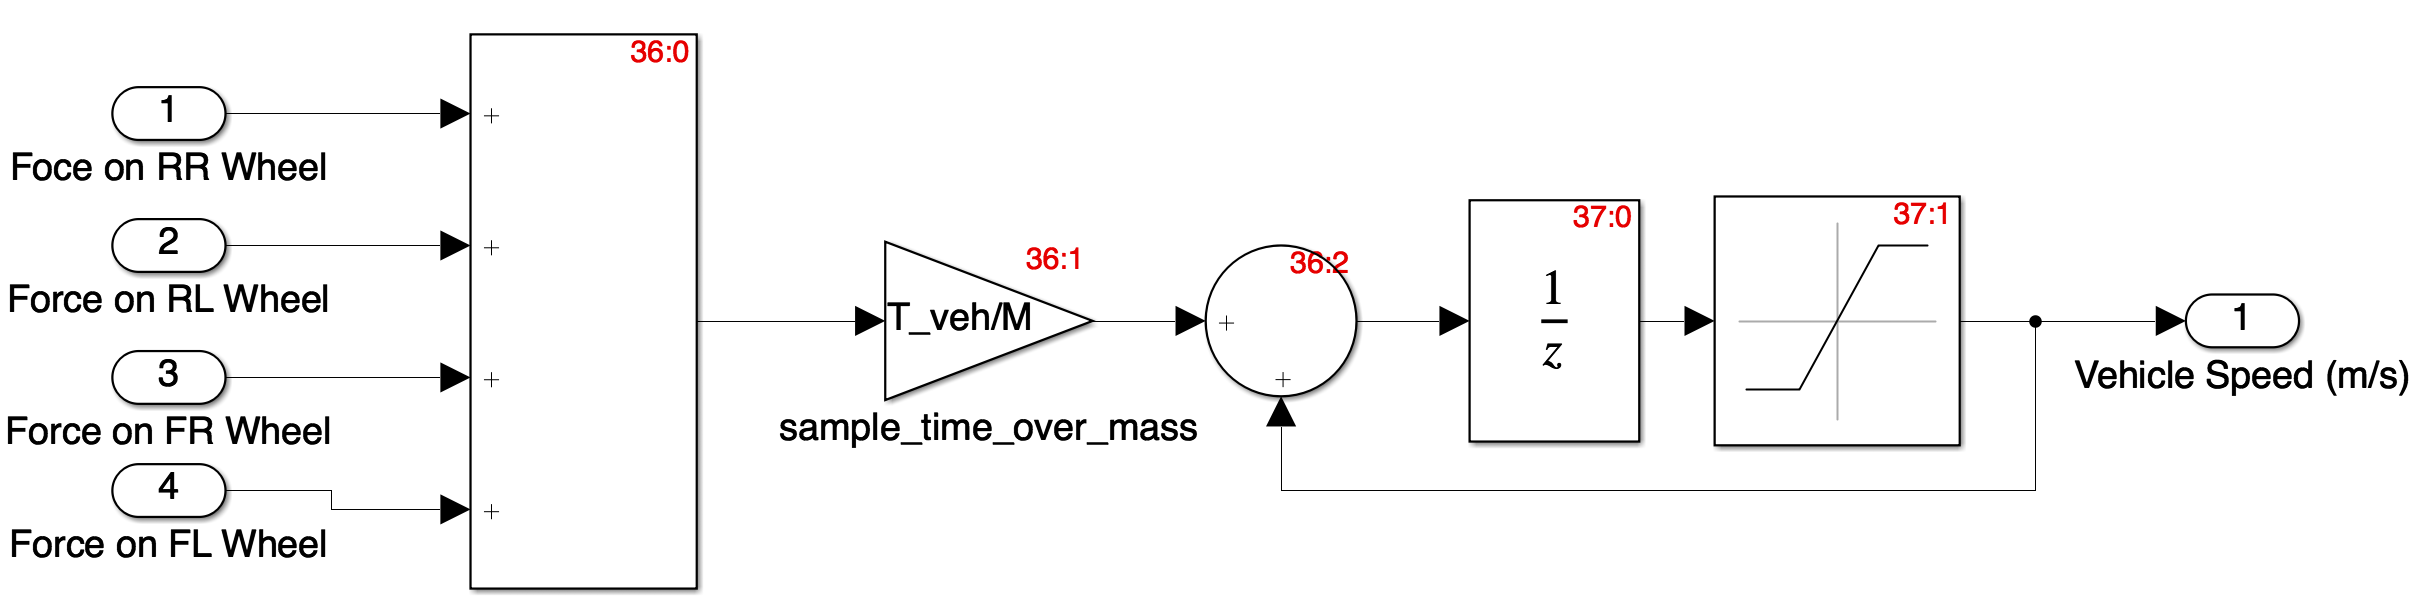
\includegraphics[width=1\linewidth]{images/sm_exec_order}
	\caption{A Subsystem block from the brake-by-wire model, computes vehicle speed. The labes in red color are indexed identifiers and denote of the execution order.}
	\label{fig_sm_exec_order}
\end{figure}

\section{Stochastic Timed Automata}
The theory of stochastic timed automata builds upon the timed automata theory via probability to support stochastic behavior in modeling and anlaysis of real-time systems. It can be used to model continuous-time behaviors, e.g., pressing the brake pedal, which occurs at continuous time points, and others, e.g., waiting time in network communication, uncertainly in input values, soft real-time deadlines. 

A timed automaton $\mathcal{A}$ is a finite-state automaton proposed by Alur et al.~\cite{Alur1999TimedAutomata} to model and anlayze real-time systems, i.e., by extending the automaton with real-valued clock variables $X$. It is widely used in the model checking to verify functional and timing requirements, e.g.,liveness, safety properties. The stochastic version automaton $\langle\mathcal{A},\mu,\gamma\rangle$ basically extends the timed automaton with probability, i.e., on the delays between states via the delay density functions $\mu$ and discrete transitions between locations via the output probability functions $\gamma$, where  $\mathcal{A}$ is represented as a tuple $\langle L,l_0,X,\Sigma,E,I\rangle$, and its elements are described as follows: $L$ is a set of locations of which $l_0$ is the initial location, $E$ is the set of edges between locations,  $\Sigma$ is a set of action labels, and $I$ is a set of invariants, which are Boolean constraints over $X$ assinged to locations, i.e., the system (or automaton) can only stay in the location as long as its invariants hold. An edge $(l,g,a,r,l')\in E$ denotes a transition relation from the location $l$ to $l'$, with conjuctions of guards $g$, action $a$ and clock resets $r$. The gaurd is also a Boolean constraint over $X$, and when it holds, the transition on the edge is enabled.
\begin{figure}
	\centering
	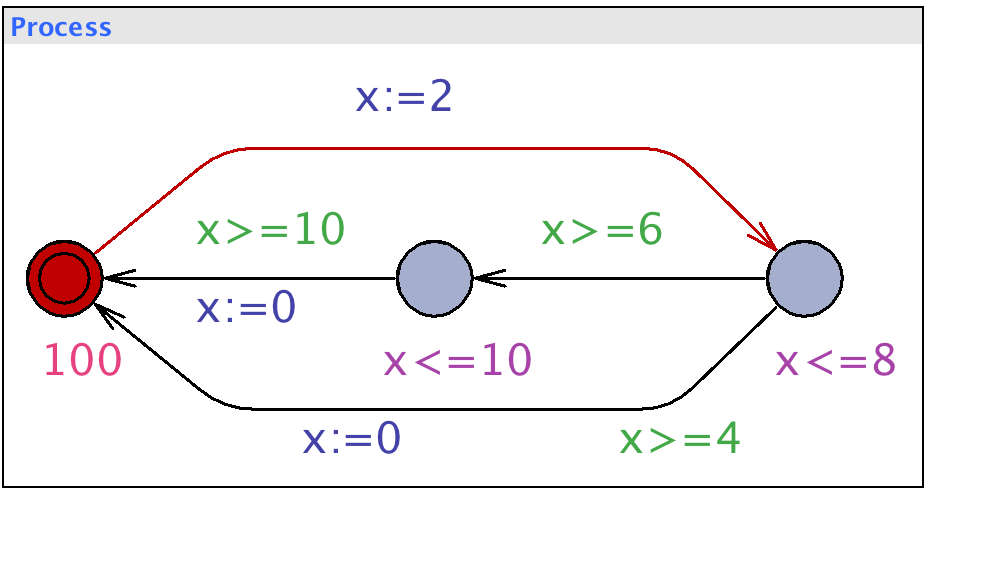
\includegraphics[width=0.6\linewidth]{images/sta_dummy_example}
	\caption{STA example.}
	\label{fig_staexample}
\end{figure}

\begin{example}[STA Example] Figure~\ref{fig_staexample} is a dummy STA example with three locations A,B and C, where A is the initial location. The guards of the automaton are labeled in Green color, the clock resets in Blue and the constraints in Red.
\end{example}

%The semantics of a timed auomaton is given as a \textit{timed transiton} system, which are abstract machines to study the computation of real-time system, and consist of states and transitions between states. 
Assume that, $d(l,v)$ is the infimum delay which satisfies the disjunction of guards on the edge that start from $l$, and assume that, $D(l,v)$ is the superimum delay which satisfies the invariant $I(l)$. If the delay is bounded, i.e., there exists $D(l,v)$, in location $l$, each delay density function in $l$, $\mu_s$, is assumed to be uniformly distributed on the interval $[d(l,v),D(l,v)]$. However, if the location is time unbounded, the delays are assumed to be exponentially distributed with the rate $R(l)$. To illustate this point, consider the same STA example, the delays at the location A are exponentially distributed, i.e., with rate 100, since the the location is time unbounded, and delays at B and C are uniformly distributed on the interval $[4,8]$ and $[10,10]$, respectively. The output probability of locations A and C is 1 and of location B is 1/2. 
%Note: logical path, and probability of taking the path is purely stochastic

\subsection*{Network of Stochastic Timed Automata}
Under the assumption of input-enabledness, disjointness of clock sets and output action sets, a network of STA (denoted by NSTA) is parallel composition of $STA_i$, i.e., $(STA||STA2||,...,||STAn)$, where n is the number of STA in the netowrk.  The state of a networked TA is a tuple $\langle s_1,s_2,...,s_n\rangle$, where $s_i=(l,v)\in L_i\times X_i$ . In NSTA, the automata communicate through broadcast channels and globally shared variables. Moreover, the semantics of the NSTA relies on the independent computation of the individual STA (or components), i.e.,  each component automaton, based on the delay density functions and the output probability functions decides repeatedly on which output to generate and at which point in time. In this race, the output will be determined by the component automaton that has chosen to produce the output after the minimum delay~\cite{David2011StatisticalAutomata}.


\section{Statistical Model Checking}
Statistical model checking uses a finite set of randomly selected execution traces (or runs) of the automata, and subsequently checks if the traces satisfies a propery $\varphi$, i.e., $S\in Runs(A)\models \varphi$. It applies statistical techniques such as hypothesis testing and mote carlo simulation the satisfaction of properties. 

UPPAAL SMC is a statistical model checker found in the UPPAAL toolset. It takes in systems that are modeled as a network of stochastic priced timed automata. In this thesis, we use the real-valued clocks $X_j$ that evolve with implicit rate 1, thus the priced automata have only stochastic semantics. In this thesis, the notion of stochastic priced timed automata is used only to model monitor automata (composed in parallel with the actual system model), whic implement the \emph{stop-watch} mechanism.

\subsection*{Properties Specification}
\uppaalsmc{} employs the probabilistic extension of \textit{weighted metric temporal logic} (WMTL) \cite{bulychev2012rewrite}, i.e., PWMTL, to describe quanitative and qualitative statistical properties, which can be inductively constructed from the following grammar:
\begin{align}
\varphi::=P(\Diamond_{c\leq t}\phi)\bowtie p | P(\Box c\leq t)\bowtie p
\end{align}
where $c$ is the observer clock of the automaton under analysis, $\phi$ is a state property, $\bowtie \in\{<, \leq, =,\geq, >\}$, and $p \in [0, 1]$.

The following types of properties can be checked in UPPAAL SMC: 
\begin{itemize}
	\item \textit{Hypothesis testing} - it is a qualitative method to check if the probability of satisfying a property $\varphi$ is less than or equal to a certain probabilistic threshold $p$ over a network of STA.
	\item \textit{Probability evaluation} - it is quantitative method to determine the probability of satisfying a certain property $\varphi$ over a network of STA.
	\item \textit{Probability comparison} - it is qualitative method to compare the probabilities of satisfying two properties $\varphi_1$ and $\varphi_2$ over a network of STA.
\end{itemize}

\section{Integer-linear Programming}
\ilp{} is an optimization problem where the decision variables are integer, and the objective function and the constraints are linear models.  They are problems that can be represented as 
\begin{align}
	&Maximize\ \sum_{j=1}^{n}{c_jx_j}\\
	\mbox{Subjec to:}&\\
	&\sum_{j=1}^n{a_ijx_j}\leq b_i&\mbox{ for all } i=1,...,m\\
	&x_j\geq 0 \land x_i\in \mathbb{I} &\mbox{ for all } i=1,...,m
\end{align}

It has many mathematical, and engineering applications, e.g., transportation, scheduling. The binary (0-1) problem is a special case of ILP where the decision variables takes on 0 or 1. It applied in several decision making problems, e.g., resource allocation in the scheduling/ assignment problem. The software mapping is an instance the assignment problem where each binary variable denote if a software component is mapped to a  processor (or computing unit) or not, i.e., 1 if assigned otherwise 0. 

ILP problems are frequently solved via exact algorithms, e.g., branch and bound, but can also be delt via heuristics, e.g., using simulated annealing, hill climbing. In this work, we use the CPLEX solver form IBM to the software-to-hardware mapping optimization.
\section{Population-based Metaheuristics}
For complex optimization problems, the ILP formulation is a difficult task and the scalability to solve large problems instances is usually prohibitively expensive. Metaheuristics~\cite{2006HandbookMetaheuristics}\cite{Gonzalez2007HandbookMetaheuristics} is a type of heuristics which uses search strategies that are sometimes less dependent on the problems and more efficient computation-wise but less optimal. Population-based metaheuristics is a class of meta-heuristic methods which uses a set of individuals (or population) in the search strategy to determine the global optima of the problem, e.g.,differential evolution~\cite{Storn1997DifferentialSpaces}\cite{Das2016RecentSurvey}, particle swarm optimization~\cite{2016ParticleOptimization}\cite{Sengupta2018ParticlePerspectivesb}.

In this work, we apply differential evolution, particle-swarm optimization to search for the best software-to-hardware mapping solution. The differential evolution employees a set of agents, which represent candidate solutions,  to find the best software-to-hardware mapping solution. Each agent applies a particular types of evolutionary operators such as mutation, crossover and selection to reach a target position in the search space. A mutant agent (or offspring) is generated for every agent and in every iteration from three other angents. If the offspring is more fit, i.e., better than the parent agent, it replaces the latter, otherwise is discarded.
\begin{align}
\label{eqn_de_mutation}
\textbf{v} & \leftarrow   \textbf{a} + F\circ(\textbf{b}-\textbf{c})\\
\label{eqn_de_crossover}
\textbf{u}&\leftarrow crossOver(\textbf{v},\textbf{x},CF,F)\\
\label{eqn_de_selection}
\textbf{x} &\leftarrow 
\begin{cases}
	\textbf{u} & \mbox{if } f(\textbf{u}) < f(\textbf{x})\mbox{ functions}\\
	\textbf{x} & \mbox{otherwise }
\end{cases}
\end{align}
where $F\in[0,2]$ is the differential weight, $CF\in[0,1]$ is the crossover probability.

Likewise, in the particle-swarm optimization, the method employs agents (in this case, particles), which are member of the population and represents candidate solutions. It records the best position of each particle so far $\textbf{p}_{bst}$ and best position of the population $\textbf{z}$. Thus, the motion of each particle is guided by its velocity, attraction towards its best position $\textbf{p}_{bst}-\textbf{p}$ and attraction towards the best position of the swarm $\textbf{z}-\textbf{p}$, where $\textbf{p}$ is a n-dimensional matrix which represents the current position of a particle in the search space.
\begin{align}
\label{eqn_pso_velocity}
\textbf{v} &\leftarrow  \omega\textbf{v} + c_1Rand()\circ(\textbf{p}_{bst}-\textbf{p}) + c_2Rand()\circ(\textbf{z}-\textbf{p})\\
\label{eqn_pso_position}
\textbf{p} &\leftarrow \textbf{p} + \textbf{v},
\end{align}
where $\omega$ is the weight of the velocity, also known as \textit{inertia coefficient} and controls the convergence of the algorithm. The $c_1, c_2$ constants are acceleration coefficients and control the weight of attraction towards the cognitive and social components, respectively. $Rand()\in U(0,1)$ is a random function along the acceleration coefficients, which is element-wise multiplied with the components to improve diversity of the search by introducing stochastic behavior